\documentclass[12pt]{amsart}

\addtolength{\hoffset}{-2.25cm}
\addtolength{\textwidth}{4.5cm}
\addtolength{\voffset}{-2.5cm}
\addtolength{\textheight}{5cm}
\setlength{\parskip}{0pt}
\setlength{\parindent}{15pt}

\usepackage{amsthm}
\usepackage{amsmath}
\usepackage{amssymb}
\usepackage[colorlinks = true, linkcolor = black, citecolor = black, final]{hyperref}

\usepackage{graphicx}
\graphicspath{ {./images/} }
\usepackage{multicol}
\usepackage{ marvosym }
\usepackage{wasysym}
\usepackage{tikz}
\usetikzlibrary{patterns}

\newcommand{\ds}{\displaystyle}
\DeclareMathOperator{\sech}{sech}

\setlength{\parindent}{0in}

\begin{document}

\thispagestyle{empty}

{\scshape Sotirios Moschos 9030} \hfill {\scshape \large Advanced Signal Processing} \hfill {\scshape Homework \#2}

\smallskip

\hrule

\bigskip

{\large\textbf{Plots}}

\bigskip

\textbf{Real discrete process X(k)}
\begin{figure}[h]
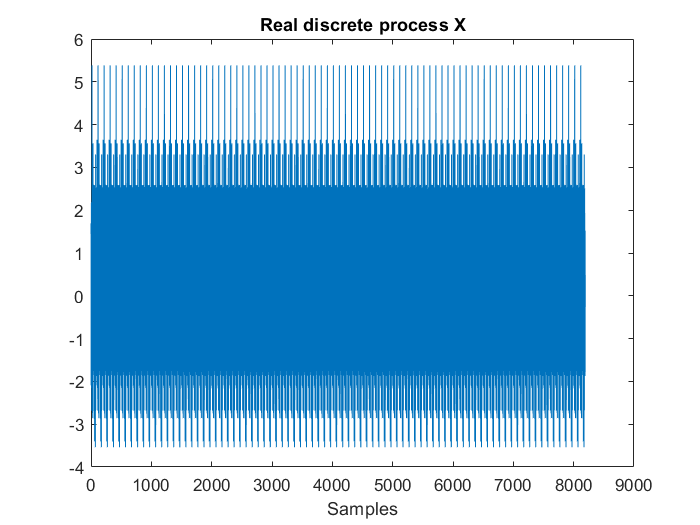
\includegraphics[width=8cm]{{Images/X(k).png}}
\end{figure}

In order to get the power spectrum we used the function SpectrumEstimator from the dsp toolbox.
We chose Welch's averaged modified periodograms method and Hann's window function.

\textbf{Power spectrum 1}
\begin{figure}[h]
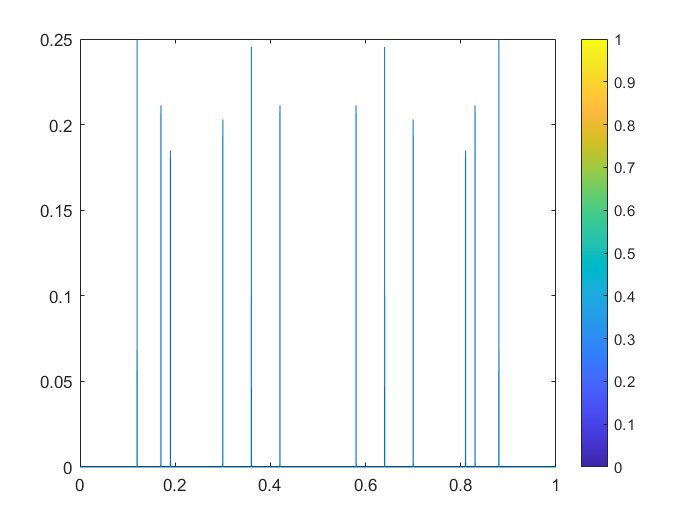
\includegraphics[width=8cm]{{Images/power spectrum 1.png}}
\end{figure}

In another approach, we calculated the the power spectrum via the FFT of the covariance of X(k). Hence, we got the following plot.

\textbf{Power spectrum 2}
\begin{figure}[h]
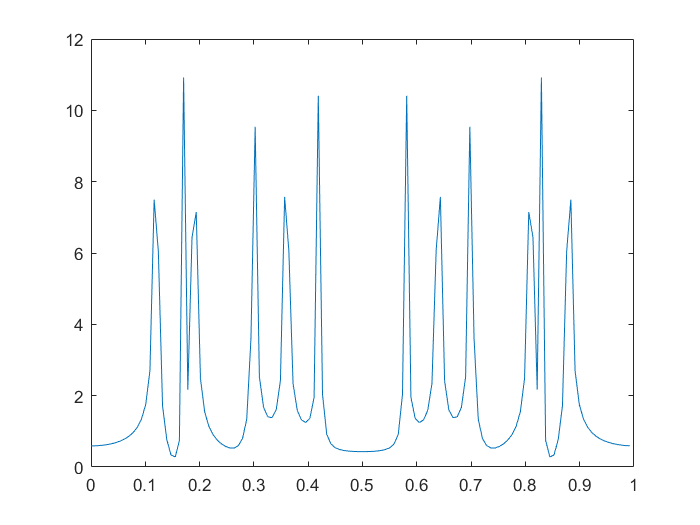
\includegraphics[width=8cm]{{Images/power spectrum 2.png}}
\end{figure}

\bigskip

{\large\textbf{Comparison of indirect bispectrum estimation methods}}

\bigskip

In order to get the following plots, we used the bispeci function from HOSA toolbox. For the first subtask we used the hexagonal window with unity values, as it's shape is similar to the rectangular window, so we can draw similar conjectures.\newline
For the second subtask we used the parzen window.\newline
Hence, we got the following plots: For the first plot we used the hexagonal window with unity values and for the second plot the parzen window.
\begin{figure}[h]
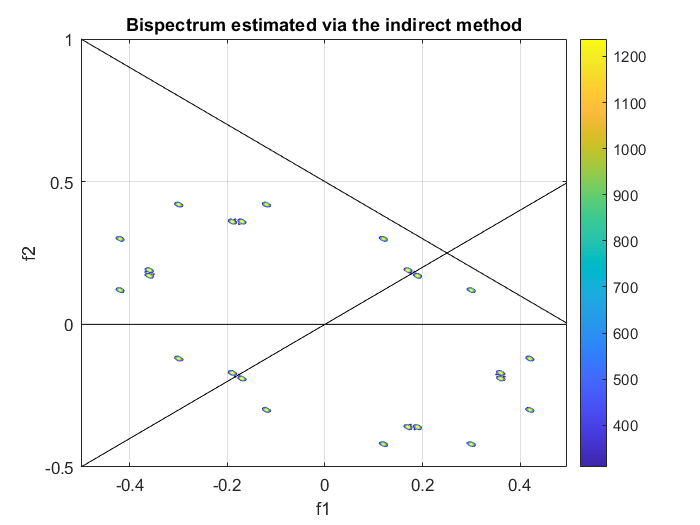
\includegraphics[width=8cm]{{Images/indirect hex.png}}
\end{figure}
\begin{figure}[h]
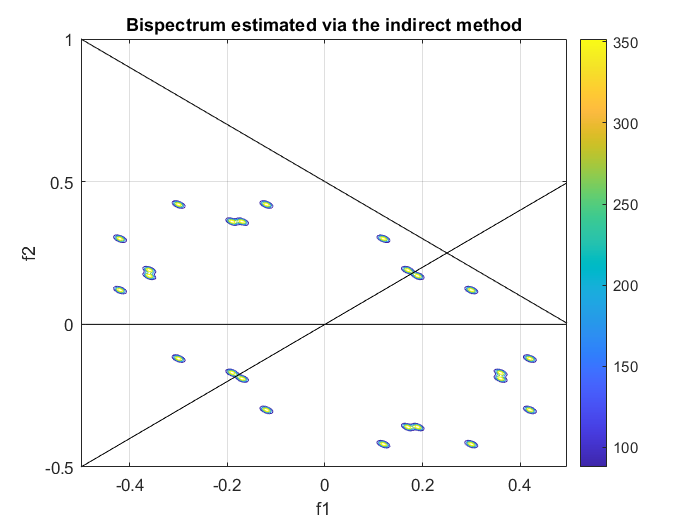
\includegraphics[width=8cm]{{Images/indirect parzen.png}}
\end{figure}

The are particular advantages and disadvantages on the use of the proper 2D window. When a finite set of measured data is available, the problem of higher-order statistics estimation for a signal is a sensible one. We should take into account the bias, the variance and other quality measures of the estimator, the bispectral resolution and finally, the leakage effect. As we can see from the plots the rectangular window has a higher frequency resolution than the Parzen window because the Parzen window offers the larger relative width of the main lobe compared to the rectangular one. The rectangular window has the larger spectral leakage effect because it has the higher sidelobe level. We obtained this information from the following paper:
(\textbf{Bispectral resolution and leakage effect of the indirect bispectrum estimate for different types of 2D window functions, 2008, Teofil-Cristian Oroian et all.}).

\bigskip
\newpage
{\large\textbf{Comparison of indirect and direct bispectrum estimation methods}}

\bigskip

In order to get the following plot, we used the bicpecd function from HOSA toolbox.
\begin{figure}[h]
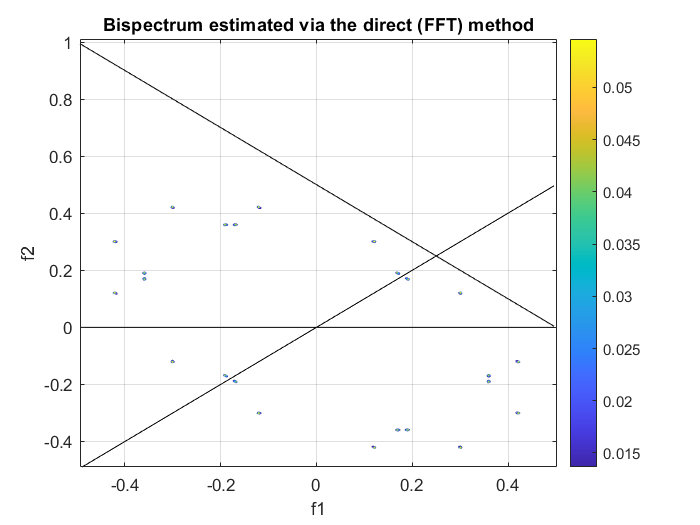
\includegraphics[width=8cm]{{Images/direct.png}}
\end{figure}\newline
We can state the the direct method has lower frequency resolution than the indirect method.

\bigskip

{\large\textbf{Frequency content of power spectrum vs bispectrum estimations}}

\bigskip

We can state that this homework assignment is a concrete application of signal processing namely, the quadratic phase coupling detection problem. In general, if we have a signal that is composed of three sinusoids with frequencies $\omega1,\omega2,\omega3$ and phases $\phi1,\phi2,\phi3$, the sinusoids 1 and 2 are said to be quadratically phase coupled (QPC) if and only if and \[\omega1+\omega2=\omega3\] \[\phi1+\phi2=\phi3\]
Analyzing the power spectrum plot, we can see that all 6 harmonics arise.
The bispectrum is a useful tool for QPC detection because only the phase couple components appear. In our case, considering the symmetries of the bispectrum we can see that frequency resolutions appear on the frequency points \[(\lambda1,\lambda2),(\lambda4,\lambda5)\] of the primary area. Thus, we can state that the sinusoids 1,2 and 4,5 are quadratically phase coupled.\newline
We obtained this information from the following paper:
(\textbf{Quadratic phase coupling phenomenon and its properties, Wieslaw Kicinski, Artur Szczepanski.}).
\bigskip

{\large\textbf{Results and plots with different segment lengths}}

\bigskip

In order to get the following plots, we changed the segment lengths from K1=32 to K2=16 and from M1=256 to M2=512 for the indirect and direct bispectrum estimations.\newline
For the first plot we used the hexagonal window with unity values and for the second plot the parzen window for the indirect bispectrum estimation.
For the third plot, we used the direct method.

\newpage

\begin{figure}[h]
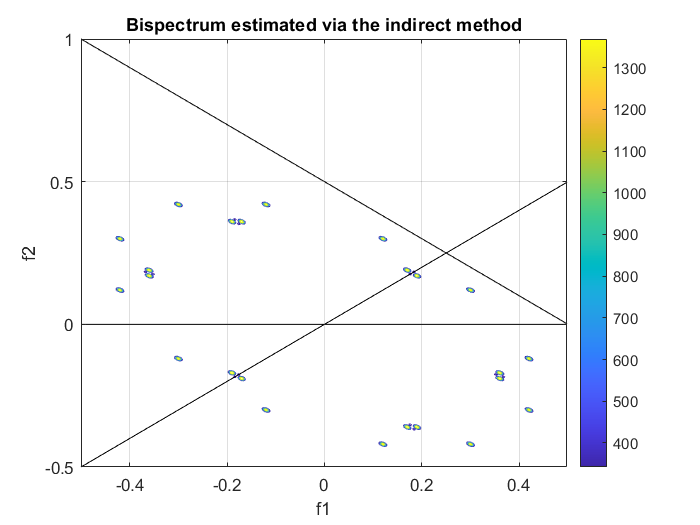
\includegraphics[width=8cm]{{Images/indirect hex K=16.png}}
\end{figure}

\begin{figure}[h]
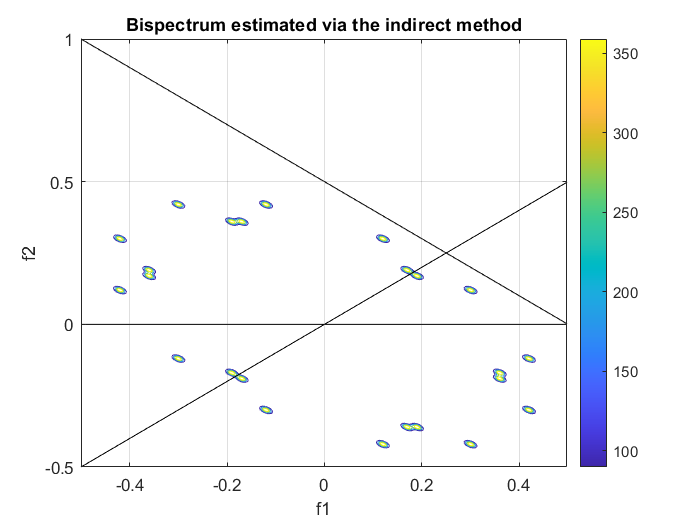
\includegraphics[width=8cm]{{Images/indirect parzen K=16.png}}
\end{figure}

\begin{figure}[h]
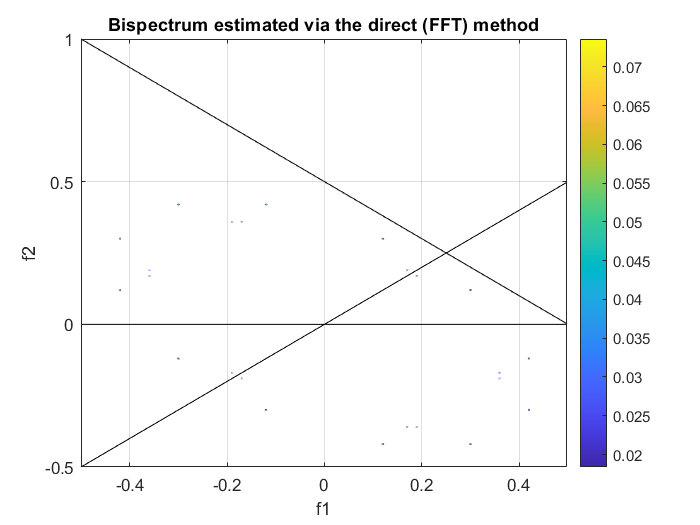
\includegraphics[width=8cm]{{Images/direct K=16.png}}
\end{figure}

From (\textbf{Bispectral resolution and leakage effect of the indirect bispectrum estimate for different types of 2D window functions, 2008, Teofil-Cristian Oroian et all.}) when the size L of the 2D window increases, the bispectral resolution is better. But, this value cannot be increasing very much because the variance of the estimator increases.

\begin{equation*}
\begin{aligned}
\sigma_3^2(\omega1,\omega2)
&= \begin{cases}
    ((V*L_3^2)/(K*M))*C_2^x(\omega1)*C_2^x(\omega2)*C_2^x(\omega1+\omega2), Indirect \\
    (N_0^2)/(K*M))*C_2^x(\omega1)*C_2^x(\omega2)*C_2^x(\omega1+\omega2), Direct \\
    0<\omega2<\omega1 \\
    \end{cases}
\end{aligned}
\end{equation*}

Hence, by increasing the window length to 512 samples we get better frequency resolution but the variance of the estimator increases.

In order to get the following plots, we changed the segment lengths from K1=32 to K3=64 and from M1=256 to M3=128 for the indirect and direct bispectrum estimations.\newline
For the first plot we used the hexagonal window with unity values and for the second plot the parzen window for the indirect bispectrum estimation.
For the third plot, we used the direct method.

\begin{figure}[h]
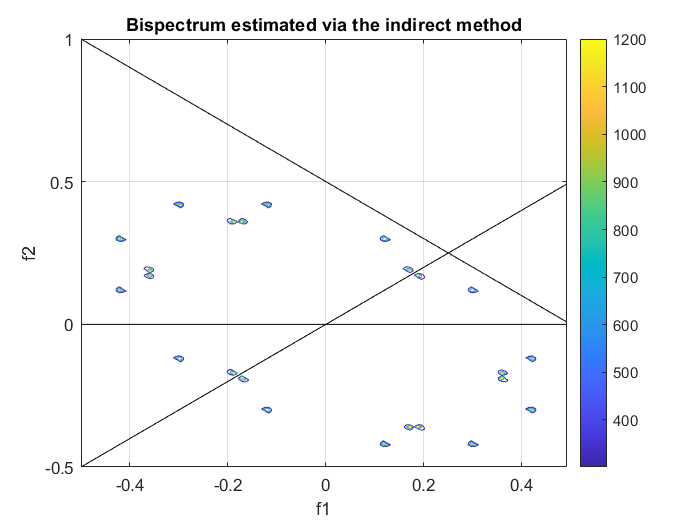
\includegraphics[width=8cm]{{Images/indirect hex K=64.png}}
\end{figure}

\begin{figure}[h]
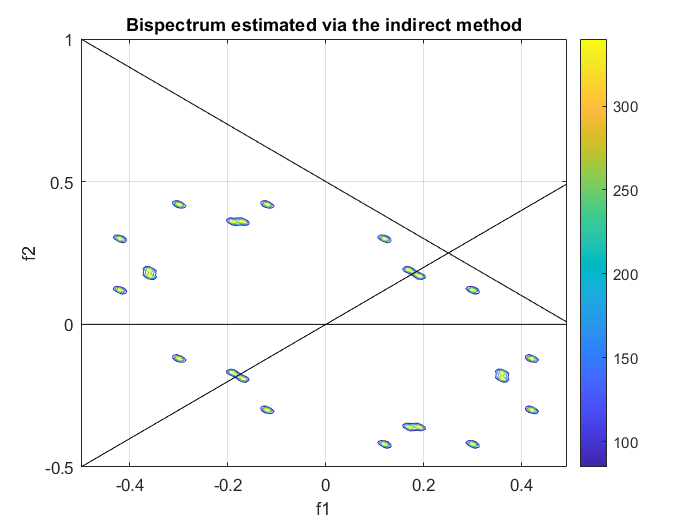
\includegraphics[width=8cm]{{Images/indirect parzen K=64.png}}
\end{figure}

\begin{figure}[h]
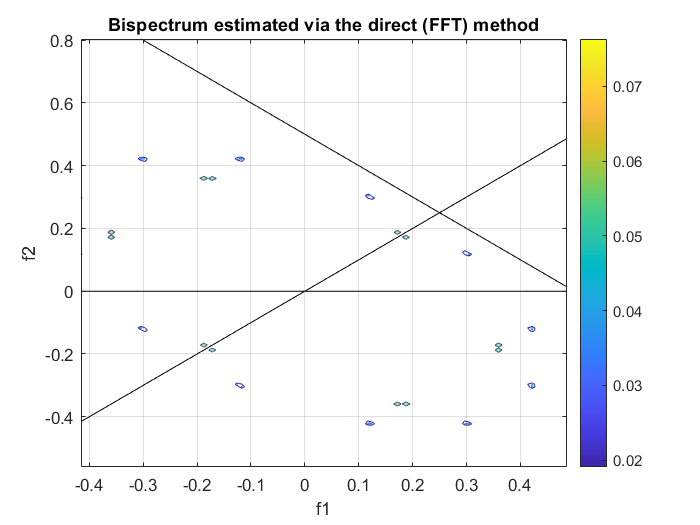
\includegraphics[width=8cm]{{Images/direct K=64.png}}
\end{figure}

Hence, by decreasing the window length to 128 samples we get lower frequency resolution and the variance of the estimator decreases.

\newpage

{\large\textbf{Mean values of estimations above for 50 realizations of X(k)}}

\bigskip

In order to get the following plots, we got 50 realizations of X(k) and we calculated the mean of the values in each frequency point to get the mean estimated power spectrum and the mean estimated bispectrum with different estimation methods. Hence, we got the following plots: \newline
The first plot is the mean power spectrum. \newline
The second plot is the mean bispectrum using the indirect method and the hexagonal window with unity values. \newline
The third plot is the mean bispectrum using the indirect method and the parzen window. \newline
The fourth plot is the mean bispectrum using the direct method. \newline

\begin{figure}[h]
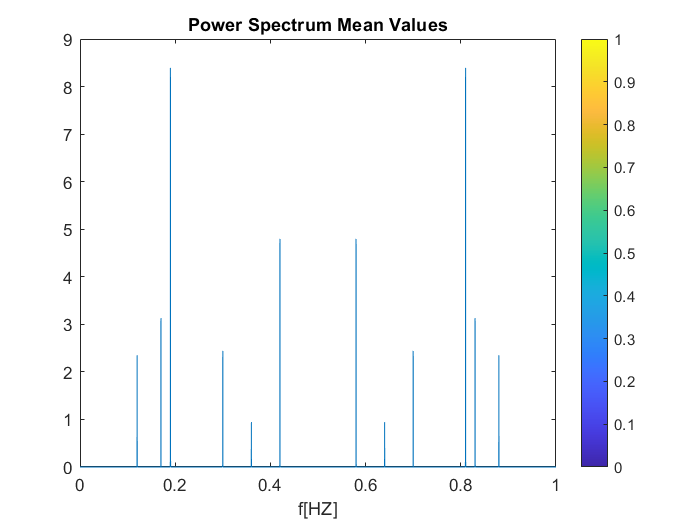
\includegraphics[width=8cm]{{Images/power spectrum 1-50.png}}
\end{figure}

\begin{figure}[h]
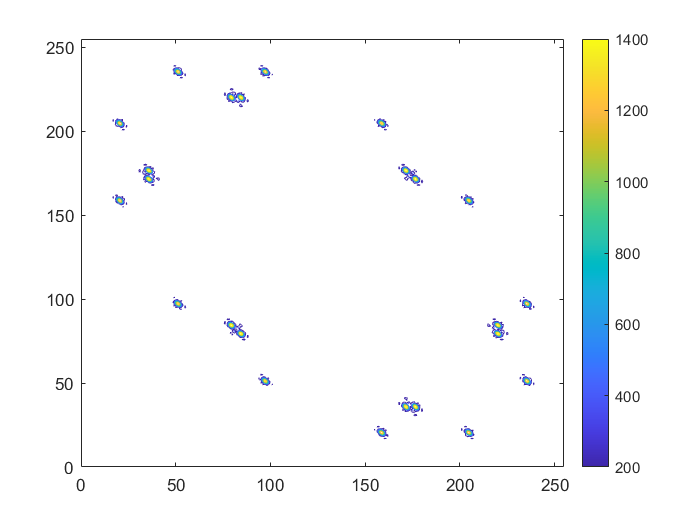
\includegraphics[width=8cm]{{Images/indirect hex-50.png}}
\end{figure}

\begin{figure}[h]
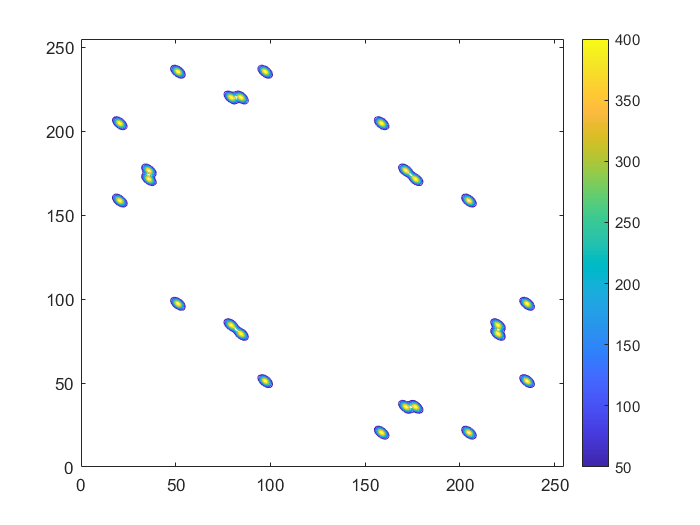
\includegraphics[width=8cm]{{Images/indirect parzen-50.png}}
\end{figure}

\begin{figure}[h]
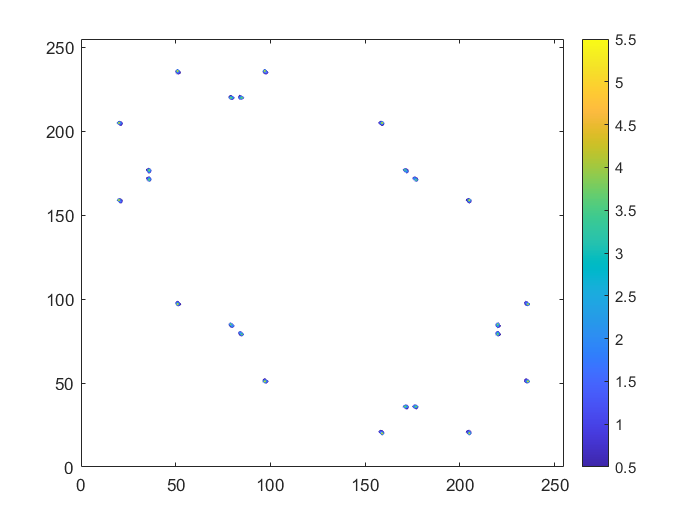
\includegraphics[width=8cm]{{Images/direct-50.png}}
\end{figure}




\end{document}
